\chapter{Background}

\section{Consensus Algorithms}

Consensus algorithms are at the core of any blockchain and are an attempt at overcoming the issue of overall system consistency despite faulty or malicious participants in a distributed, trust-less environment. The primary obstacle of blockchains that consensus algorithms are designed to solve is the Byzantine Generals Problem \cite{lamportshostakpease1982}: a scenario in which allied generals ---geographically separated by the enemy--- are attempting to communicate without the message being caught and tampered with. As a distributed system, data sent over the network is never guaranteed to reach their destination and can be intercepted by malicious actors. Hence, a strategy is required to both ensure the integrity of the chain, and ensure that the correct version is received by as many participants as possible.

\subsection{Proof of Work (PoW)} \label{section:pow} 

PoW overcomes the aforementioned issue using a variation of HashCash \cite{back2002} by creating a cryptographic puzzle with merkle trees that is computationally expensive with the solution used as verification for the next block. Attempting to rewrite history or faking blocks requires having enough computational power to solve the puzzles of each related block and overtake the creation of the next block, creating a chain that is longer than the honest chain.

\subsection{Mining}

Each block on a blockchain contains a timestamp, verified transactions, and most importantly a cryptographic hash of the previous block which facilitates the chaining. The process of mining a block is designed to be prohibitively difficult and aims to be solvable in a consistent time. It involves several components:

\begin{itemize}
  \item $T$ A collection of unverified transactions (not yet on the blockchain)
  \item $t$ - The digest of a merkle tree created from $T$
  \item $h_p$ - The hash of the previous block.
  \item $n$ - A random string otherwise known as the \textit{nonce}.
  \item $\lambda$ - The difficulty of the puzzle (where $\lambda > 1$) where $\lambda$ is the required number of zeroes padding the solution (changes every 2016 blocks).
  \item $\mathbb{H}$ - The hash function chosen by the miner that outputs 256 bits based on the input.
  \item $H$ - Hash rate of the miner, the number of times $\mathbb{H}$ can be executed per second.
\end{itemize}

The miner is required to verify transactions $T$ and \textit{pack} them by hashing them into a merkle tree. Then, they must create a suitable hash for the block. A potential hash is found via the function $h = \mathbb{H}(t \| h_p \| n)$ with each attempt changing $n$ (and occasionally $t$). When an appropriate nonce is chosen, $h$ should satisfy the condition $h \leq \frac{2^{256}}{\lambda}$ to be a suitable solution. The difficulty $\lambda$ is chosen such that the computational work necessary to solve the problem will require the full block time. That is in $\frac{\lambda \times 2^{32}}{h}$ seconds based on the average hash rate of the last 2016 blocks \cite{difficulty2019}.

\subsection{Difficulty}

Given a hash is a number between 0 and $2^{256}-1$, and the difficulty as of Nov 1 2020 at 19997335994446.11 \cite{chainquery2020}, the expected number of hashes to validate a block can be approximated \cite{difficulty2019} with:

\begin{align}
    H &= \frac{\lambda \times 2^{32}}{600} \\
    &= \frac{19997335994446.11 \times 2^{32}}{600} \\
    & \approx \text{14EH/s}
\end{align} 

The expected time to validate a block for an individual miner with an Antminer S19 Pro at 110 TH/s \cite{antminer2018} can be estimated \cite{difficulty2019} with:

\begin{align}
    t &= \frac{\lambda \times 2^{32}}{h} \\
    &= \frac{19997335994446.11 \times 2^{32}}{110e12} \\
    & \approx 1301331.8 \text{ blocks} \\
    & \approx 24.6 \text{ years}
\end{align}

The miner would be contributing $\frac{110e12}{14e18} = 7.8e{^-8}\%$ of the global hash rate. If it is assumed the miner eventually succeeds in mining a block, distributing their reward over all unsuccessful blocks yields an amortised profit of $\frac{12.5}{1301331.8} \approx 9.6e{^-6} \text{\bitcoin}$. However, it is unreasonable to assume the difficulty and hash rate be constant, nor is it likely a miner would be able to finance their operating costs on a long-term high risk investment considering the volatility of the cryptocurrency market.

\section{Mining Pools}

While the intention of PoW is for each participant mine individually for a truly decentralised implementation, there is no punishment for collusion, nor is behaving honestly always the most profitable method of participation. Since most miners are incentivised by profit rather than maintaining the integrity of the blockchain they will seek to increase their hash rate for a better chance at the reward. However, as the global hash rate increases, the difficulty is adjusted to control block creation speed. In response to the increased difficulty, miners have formed coalitions to pool their resources. Both work and rewards are delegated to participants. While the amount would be very similar to mining individually, the variance of payout is reduced. Supposing the aforementioned miner joins a pool with an estimated 4EH/s of computational power, the pool would expect to receive a reward in 35.7 blocks or 5.9 hours with an amortised reward of $0.35\text{\bitcoin}$ per block. With the miner contributing $\frac{110e12}{4e18} \approx 2.8e{^-5}\%$, they would expect to receive the same $9.6e{^-6} \text{\bitcoin}$ per block.

As of 1 Nov 2020, the hash rate distribution is seen in \cref{figure:hashrate-distribution} below. The data used to create the chart can be found in \cref{appendix:hashrate-distribution}.

\begin{figure}[H]
  \centering
  \caption{Hash rate distribution over a 24 hour period}
  \label{figure:hashrate-distribution}
  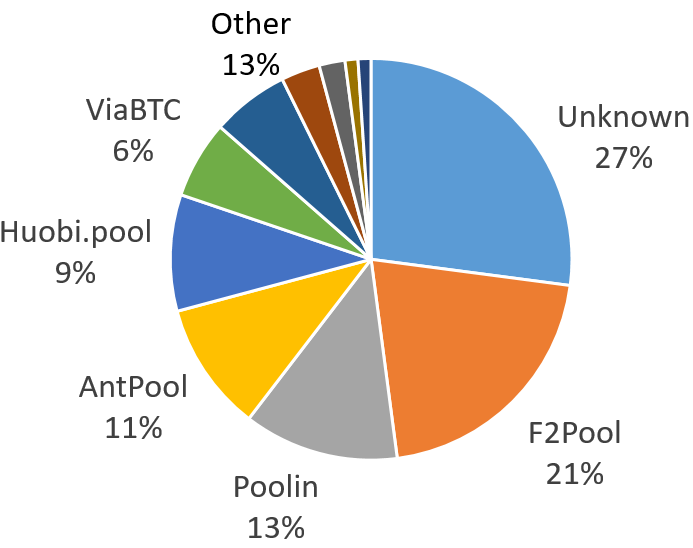
\includegraphics[scale=0.5]{media/hashrate-distribution.PNG}
\end{figure}

While a \textit{sufficiently} distributed network may mean that the computational power of an entity should never exceed 50\% or more of the global hash rate, a higher degree of fragmentation would be preferred for a truly secure network.

\section{Harberger Tax}
\label{section:harberger-tax}

The Harberger Tax \cite{posnerweyl2017} is an economic policy that aims to prevent unequal distribution of property through two rules:

\begin{itemize}
  \item Owners assign a self-assessed value to their property and pay a proportional tax.
  \item The owner is unable to prevent anybody from purchasing their property at their previously set price.
\end{itemize}

The purpose of the first rule is to discourage owners from monopolising their property by assigning a prohibitively high price to prevent others from purchasing as they themselves would have to shoulder the proportional tax. The next rule ensures the mobility of property and that there is no incentive to invest in their property as it is likely to be taken at any given point. This combats the issue of price inflation where an owner may ``hold" their property and increase demand and inflate the price. It will also ensure owners do not set their price too low to avoid taxation.

\section{Strategic Game}
\label{section:strategic-game}

A model can be considered a strategic game if it consists of a finite set of decision-makers $N$ from which each decision-maker has a non-empty set of action profiles $A_i$ that are non-revocable and will be executed simultaneously based on associated preferences \cite[Section 2.1]{osborne1994}. A key factor is that each decision-maker's preferences must also take into account all possible decisions in the game. This definition can be applied to a wide variety of scenarios including the economic model in this proposal, with participants acting as the decision-makers, and their actions being based on not only their own circumstances, but also the actions of other participants.

Once players and their strategies are defined, a table can be constructed in the following format:

\begin{table}[H]
  \centering
  \caption{Example of a finite game with two players}
  \label{table:nashexample}
  \begin{tabular}{|l||*{5}{c|}}\hline
    \backslashbox{Player A}{Player B} & \makebox{Strategy 1} & \makebox{Strategy 2} \\
    \hline \hline
    Strategy 1                        & $a_1$, $b_1$         & $a_1$, $b_2$         \\ \hline
    Strategy 2                        & $a_2$, $b_1$         & $a_2$, $b_2$         \\ \hline
  \end{tabular}
\end{table}

From \cref{table:nashexample}, each cell represents a game in which Player A and Player B each chose a particular strategy which results in a \textit{payoff function} that represents the outcome of the game if the decisions in that cell were taken.

\subsection{Nash Equilibrium} \label{section:nash}

Given a strategic game as defined in \cref{section:strategic-game}, the Nash equilibrium is the proposed \textit{steady state} in which all players are acting based on the \textit{best decision} they can while aware of the actions their opponent(s) will take \cite[Section 2.2]{osborne1994}. Once the strategies of all players, the possible decisions, and all possible game states are defined (at least in natural language) according to the requirements of a strategic game, a Nash equilibrium exists for any action profile in which all players make a decision such that no player can make a decision that results in an outcome more preferred than the current game state. Determining the Nash equilibrium may yield strategies to ensure participants are not incentivised to deviate from the expected behaviour and gain an unfair advantage. 

\subsection{Auctions} \label{section:auctions}

An auction can be considered a strategic game with players, each with a set of strategies and corresponding payoffs for strategy combinations. There are multiple types of auctions \cite{auctions1987} but the most common are:

\begin{itemize}
    \item First price sealed bid auction - Bidders each make a single private bid simultaneously. The highest bidder wins and pays the amount bid.
    \item Second price sealed bid auction - Similar to first price sealed bid, however the highest bidder pays the second highest amount bid.
    \item Open ascending auction - Bidders make increasingly higher bids, until no bidder is willing to pay more.
    \item Open descending bid auction - The price is set excessively high and gradually lowered until a bidder is willing to pay the amount.
\end{itemize}

The bidders themselves are generally modelled with the following factors in mind that may be relaxed to introduce variation in the auction:

\begin{itemize}
    \item Risk-adversity - Bidders would be more or less likely to bid higher on an item given how risk-averse they are.
    \item Information - All bidders should have equal access to information.
    \item Valuation - Each bidder holds the item at a different value individually based on a probability distribution.
    \item Payment - No incentives or royalties are factors in the valuation of the item.
\end{itemize}

\section{Markov Chains}

Markov chains are used to model stochastic systems through a set of states and transitions in either a discrete or continuous time state space. To be eligible for modelling with a Markov chain, a system must be predictable no matter it's current state (i.e. memoryless) \cite{karlin2012first}. In other words, each outgoing transition $t$ from a state $X_n$ has an associated probability that must be based purely on the information present in the state. The probability distributions given by the transitions may then be used to determine the reachability of a state $X_n$ through a set of transitions (or path) $S_t = \{t_0, t_1, \ldots, t_n\}$ with $P(X_n) = \prod_{i=0}^n P(t_i)$.

\section{Related Work}

Two Phase PoW \cite{bastiaan2015} introduces an additional puzzle that requires the use of a private key to sign the work done. While this method would discourage outsourcing, it essentially negates any possibility of public pools that miners rely on for reduced variance. 

P2Pool \cite{p2pool} is an attempt at creating a completely decentralised mining pool (i.e. without a supervisor) but it is riddled with technical issues, high overhead, and much higher variance compared to other pools. 

Smartpool \cite{smartpool2017} is another proposed solution in which the pool is orchestrated via a smart contract (a self-executing ) on the Ethereum blockchain. This is a valid solution that may solve the centralisation of authority for public pools, however there is no incentive for private pools to utilise such a method. 

NiceHash and many other similar platforms, are cryptocurrency hash power brokers in which members can rent hashing power to contribute to a pool of their choice. They make no attempts to address the issue of authority centralisation, rather, their platform enables and encourages it.
